

%% NJCTL: PSI AP Physics C
%%----------------------------------------


%% Momentum
%%----------------------------------------
\element{njctl}{
\begin{question}{momentum-Q01}
    A steel ball and a piece of clay have equal mass.
    They are dropped from the same height on a horizontal steel platform.
    The ball bounces back with nearly the same speed with which it hit.
    The clay sticks to the platform.
    Which object experiences the greater momentum change?
    \begin{choices}
      \correctchoice{the ball}
        \wrongchoice{the clay}
        \wrongchoice{Both experience the same momentum change}
        \wrongchoice{there is no momentum change for either}
        \wrongchoice{more information is required}
    \end{choices}
\end{question}
}

\element{njctl}{
\begin{question}{momentum-Q02}
    A car of mass $m$ is moving with a momentum $p$.
    How would you represent its kinetic energy in terms of these two quantities?
    \begin{multicols}{3}
    \begin{choices}
      \correctchoice{$\dfrac{p^2}{2m}$}
        \wrongchoice{$\dfrac{1}{2} mp^2$}
        \wrongchoice{$mp$}
        \wrongchoice{$\dfrac{mp}{2}$}
        \wrongchoice{zero}
    \end{choices}
    \end{multicols}
\end{question}
}

\element{njctl}{
\begin{question}{momentum-Q03}
    A bowling ball moving with speed $v$ collides head-on with a stationary tennis ball.
    The collision is elastic,
        and there is no friction.
    The bowling ball barely slows down.
    What is the speed of the tennis ball after the collision?
    \begin{multicols}{2}
    \begin{choices}
        \wrongchoice{nearly $v$}
      \correctchoice{nearly $2v$}
        \wrongchoice{nearly $3v$}
        \wrongchoice{nearly infinite}
        \wrongchoice{Zero}
    \end{choices}
    \end{multicols}
\end{question}
}

\element{njctl}{
\begin{question}{momentum-Q04}
    An object with a mass of \SI{2}{\kilo\gram} is accelerated from rest.
    The graph shows the magnitude of the net force as a function of time.
    \begin{center}
    \begin{tikzpicture}
        \begin{axis}[
            axis y line=left,
            axis x line=bottom,
            axis line style={->},
            xlabel={time},
            x unit=\si{\second},
            xtick={0,2,4},
            minor x tick num=1,
            ylabel={force},
            y unit=\si{\newton},
            ytick={0,1,2},
            minor y tick num=1,
            xmin=0,xmax=4.25,
            ymin=0,ymax=2.25,
            width=0.8\columnwidth,
            height=0.5\columnwidth,
            grid=both,
            very thin,
        ]
        \addplot[line width=1pt,domain=0:4.5]{0.5*x};
        \end{axis}
    \end{tikzpicture}
    \end{center}
    At $t=\SI{4}{\second}$,
        the object's velocity would have been closest to which of the following?
    \begin{multicols}{2}
    \begin{choices}
      \correctchoice{\SI{2}{\meter\per\second}}
        \wrongchoice{\SI{4}{\meter\per\second}}
        \wrongchoice{\SI{10}{\meter\per\second}}
        \wrongchoice{\SI{13}{\meter\per\second}}
        \wrongchoice{cannot be determined}
    \end{choices}
    \end{multicols}
\end{question}
}

\element{njctl}{
\begin{question}{momentum-Q05}
    A \SI{3}{\kilo\gram} ball is dropped onto a concrete floor.
    What is the magnitude of the ball's change in momentum if its speed just before striking the floor is \SI{7}{\meter\per\second} and its rebound speed is \SI{3}{\meter\per\second}?
    \begin{multicols}{2}
    \begin{choices}
        \wrongchoice{\SI{10}{\kilo\gram\meter\per\second}}
        \wrongchoice{\SI{15}{\kilo\gram\meter\per\second}}
      \correctchoice{\SI{30}{\kilo\gram\meter\per\second}}
        \wrongchoice{\SI{50}{\kilo\gram\meter\per\second}}
        \wrongchoice{\SI{70}{\kilo\gram\meter\per\second}}
    \end{choices}
    \end{multicols}
\end{question}
}

\newcommand{\PSIapcMomentumQSix}{
\begin{tikzpicture}
    %% Ground
    \node[anchor=north,fill,pattern=north east lines,minimum width=6cm, minimum height=0.05cm] at (0,0) {};
    \draw (-3,0) -- (3,0);
    %% Mass
    \node[draw,fill=white!90!black,minimum size=1cm,anchor=south] (A) at (-2,0) {$m$};
    \node[draw,fill=white!90!black,minimum size=1cm,anchor=south] (B) at (+2,0) {$m$};
    %% Vectors
    \draw[thick,->] (B.west) -- ++(180:1cm) node[anchor=south,pos=0.5] {$4v$};
    %% Labels
    \node[anchor=south] at (A.north) {Block 2};
    \node[anchor=south] at (B.north) {Block 1};
\end{tikzpicture}
}

\element{njctl}{
\begin{question}{momentum-Q06}
    %% Questions 6-8 tikz
    Two blocks are on a frictionless surface and have the same mass $m$.
    Block 2 is initially at rest.
    Block 1 moves to the left with speed $4v$.
    Block 1 collides inelastically with block 2.
    \begin{center}
        \PSIapcMomentumQSix
    \end{center}
    Which of the following choices is closest to the final speed of the system of two blocks?
    \begin{multicols}{3}
    \begin{choices}
        \wrongchoice{$v$}
      \correctchoice{$2v$}
        \wrongchoice{$3v$}
        \wrongchoice{$4v$}
        \wrongchoice{$5v$}
    \end{choices}
    \end{multicols}
\end{question}
}

\element{njctl}{
\begin{question}{momentum-Q07}
    %% Questions 6-8 tikz
    Two blocks are on a frictionless surface and have the same mass $m$.
    Block 2 is initially at rest.
    Block 1 moves to the left with speed $4v$.
    Block 1 collides elastically with block 2.
    \begin{center}
        \PSIapcMomentumQSix
    \end{center}
    What is the final speed of block 1?
    \begin{multicols}{3}
    \begin{choices}
      \correctchoice{zero}
        \wrongchoice{$v$}
        \wrongchoice{$2v$}
        \wrongchoice{$3v$}
        \wrongchoice{$4v$}
    \end{choices}
    \end{multicols}
\end{question}
}

\element{njctl}{
\begin{question}{momentum-Q08}
    %% Questions 6-8 tikz
    Two blocks are on a frictionless surface and have the same mass $m$.
    Block 2 is initially at rest.
    Block 1 moves to the left with speed $4v$.
    Block 1 collides elastically with block 2.
    \begin{center}
        \PSIapcMomentumQSix
    \end{center}
    What is the final speed of block 2?
    \begin{multicols}{3}
    \begin{choices}
        \wrongchoice{$v$}
        \wrongchoice{$2v$}
        \wrongchoice{$3v$}
      \correctchoice{$4v$}
        \wrongchoice{$6v$}
    \end{choices}
    \end{multicols}
\end{question}
}

\element{njctl}{
\begin{question}{momentum-Q09}
    %%Questions 9-10
    A hockey stick hitting a \SI{0.5}{\kilo\gram} puck is in contact with the puck for a time of \SI{0.05}{\second}.
    The puck travels in a straight line as it approaches and then leaves the hockey stick.
    %% Start question
    If the puck arrives at the stick with a velocity of \SI{6.4}{\meter\per\second} and leaves with a velocity of \SI{-3.6}{\meter\per\second},
        what is the magnitude of the change in momentum of the puck?
    \begin{multicols}{3}
    \begin{choices}
        \wrongchoice{\SI{2}{\kilo\gram\meter\per\second}}
        \wrongchoice{\SI{3}{\kilo\gram\meter\per\second}}
      \correctchoice{\SI{5}{\kilo\gram\meter\per\second}}
        \wrongchoice{\SI{6}{\kilo\gram\meter\per\second}}
        \wrongchoice{\SI{10}{\kilo\gram\meter\per\second}}
    \end{choices}
    \end{multicols}
\end{question}
}

\element{njctl}{
\begin{question}{momentum-Q10}
    %%Questions 9-10
    A hockey stick hitting a \SI{0.5}{\kilo\gram} puck is in contact with the puck for a time of \SI{0.05}{\second}.
    The puck travels in a straight line as it approaches and then leaves the hockey stick.
    %% Start question
    If the puck arrives at the stick with a velocity of \SI{6.4}{\meter\per\second} and leaves with a velocity of \SI{-3.6}{\meter\per\second},
        what is the magnitude of the average force acting on the puck?
    \begin{multicols}{3}
    \begin{choices}
      \correctchoice{\SI{100}{\newton}}
        \wrongchoice{\SI{150}{\newton}}
        \wrongchoice{\SI{200}{\newton}}
        \wrongchoice{\SI{300}{\newton}}
        \wrongchoice{\SI{500}{\newton}}
    \end{choices}
    \end{multicols}
\end{question}
}

\newcommand{\PSIapcMomentumQEleven}{
\begin{tikzpicture}
    \begin{axis}[
        axis y line=left,
        axis x line=bottom,
        axis line style={->},
        xlabel={time},
        x unit=\si{\second},
        xtick={0,2,4,6},
        minor x tick num=1,
        ylabel={force},
        y unit=\si{\newton},
        ytick={0,2,4,6},
        minor y tick num=1,
        xmin=0,xmax=6.5,
        ymin=0,ymax=6.5,
        width=0.8\columnwidth,
        height=0.5\columnwidth,
        grid=both,
        very thin,
    ]
    \addplot[line width=1pt,mark=\empty] plot coordinates {(0,6) (4,6) (6,0) };
    \end{axis}
\end{tikzpicture}
}

\element{njctl}{
\begin{question}{momentum-Q11}
    %% Questions 11-12
    An object of mass \SI{3}{\kilo\gram} starts from rest and moves along the $x$-axis.
    A net horizontal force is applied to the object in the $+x$ direction, as shown below.
    \begin{center}
        \PSIapcMomentumQEleven
    \end{center}
    What is the net impulse delivered by this force?
    \begin{multicols}{3}
    \begin{choices}
        \wrongchoice{\SI{6}{\newton\second}}
        \wrongchoice{\SI{8}{\newton\second}}
        \wrongchoice{\SI{24}{\newton\second}}
      \correctchoice{\SI{30}{\newton\second}}
        \wrongchoice{\SI{36}{\newton\second}}
    \end{choices}
    \end{multicols}
\end{question}
}

\element{njctl}{
\begin{question}{momentum-Q12}
    %% Questions 11-12
    An object of mass \SI{3}{\kilo\gram} starts from rest and moves along the $x$-axis.
    A net horizontal force is applied to the object in the $+x$ direction, as shown below.
    \begin{center}
        \PSIapcMomentumQEleven
    \end{center}
    What is the net work done on the object?
    \begin{multicols}{3}
    \begin{choices}
        \wrongchoice{\SI{30}{\joule}}
        \wrongchoice{\SI{50}{\joule}}
        \wrongchoice{\SI{90}{\joule}}
      \correctchoice{\SI{150}{\joule}}
        \wrongchoice{\SI{120}{\joule}}
    \end{choices}
    \end{multicols}
\end{question}
}

\element{njctl}{
\begin{question}{momentum-Q13}
    A tennis ball of mass $m$ rebounds from a vertical wall with the same speed $v$ as it had initially.
    \begin{center}
    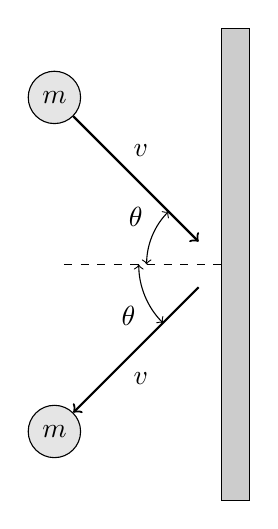
\begin{tikzpicture}
        %% Wall
        \draw[fill=white!80!black] (0,-3) rectangle  (1em,3);
        %% Normal and Angle
        \draw[dashed] (-2,0) -- (0,0);
        \draw[<->] (-0.95,0) arc(180:135:0.95) node[pos=0.5,anchor=south east] {$\theta$};
        \draw[<->] (-1.05,0) arc(180:225:1.05) node[pos=0.5,anchor=north east] {$\theta$};
        %% Balls
        \node[draw,circle,fill=white!90!black] (A) at (135:3) {$m$};
        \node[draw,circle,fill=white!90!black] (B) at (225:3) {$m$};
        %% Velocity
        \draw[thick,->] (A.south east) -- ++(-45:2.25) node[pos=0.4,anchor=south west] {$v$};
        \draw[thick,<-] (B.north east) -- ++(+45:2.25) node[pos=0.4,anchor=north west] {$v$};
    \end{tikzpicture}
    \end{center}
    What is the change in momentum of the ball?
    \begin{multicols}{3}
    \begin{choices}
        \wrongchoice{$mv$}
        \wrongchoice{$2mv$}
      \correctchoice{$2mv\cos\theta$}
        \wrongchoice{$2mv\sin\theta$}
        \wrongchoice{zero}
    \end{choices}
    \end{multicols}
\end{question}
}

\element{njctl}{
\begin{question}{momentum-Q14}
    A steel ball moving at a constant speed $v$ on a horizontal frictionless surface collides obliquely with an identical ball initially at rest.
    The velocity of the first ball before and after the collision is presented in the below diagram.
    \begin{center}
    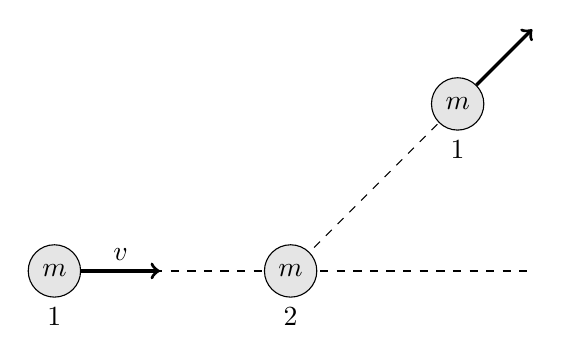
\begin{tikzpicture}
        %% lines
        \draw[dashed] (-3,0) -- (3,0);
        \draw[dashed] (0,0) -- (3,3);
        %% Three Ball
        \node[draw,circle,fill=white!90!black] (A) at (180:3) {$m$};
        \node[draw,circle,fill=white!90!black] (B) at (0,0) {$m$};
        \node[draw,circle,fill=white!90!black] (C) at (45:3) {$m$};
        %% Labels
        \node[anchor=north] at (A.south) {$1$};
        \node[anchor=north] at (B.south) {$2$};
        \node[anchor=north] at (C.south) {$1$};
        %% Vectors
        \draw[very thick,->] (A.east) -- ++(0:1) node[pos=0.5,anchor=south] {$v$};
        \draw[very thick,->] (C.north east) -- ++(45:1);
    \end{tikzpicture}
    \end{center}
    What is the approximate direction of the velocity of the second ball after the collision?
    \begin{multicols}{3}
    \begin{choices}
        \AMCboxDimensions{down=-0.4cm}
        \wrongchoice{
            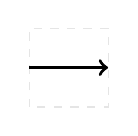
\begin{tikzpicture}
                \draw[white!90!black,dashed] (0,0) rectangle (1,1);
                \draw[very thick,->] (0,0.5) -- (1,0.5);
            \end{tikzpicture}
        }
        \wrongchoice{
            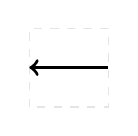
\begin{tikzpicture}
                \draw[white!90!black,dashed] (0,0) rectangle (1,1);
                \draw[very thick,->] (1,0.5) -- (0,0.5);
            \end{tikzpicture}
        }
        \correctchoice{
            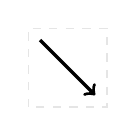
\begin{tikzpicture}
                \draw[white!90!black,dashed] (0,0) rectangle (1,1);
                \draw[very thick,->] (0.15,0.85) -- (0.85,0.15);
            \end{tikzpicture}
        }
        \wrongchoice{
            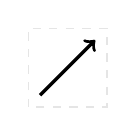
\begin{tikzpicture}
                \draw[white!90!black,dashed] (0,0) rectangle (1,1);
                \draw[very thick,->] (0.15,0.15) -- (0.85,0.85);
            \end{tikzpicture}
        }
        \wrongchoice{
            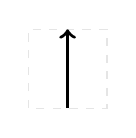
\begin{tikzpicture}
                \draw[white!90!black,dashed] (0,0) rectangle (1,1);
                \draw[very thick,->] (0.5,0) -- (0.5,1);
            \end{tikzpicture}
        }
    \end{choices}
    \end{multicols}
\end{question}
}

%% NOTE: reuse for work performed on pieces
\newcommand{\PSIapcMomentumQFifteen}{
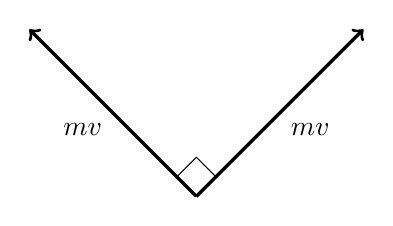
\begin{tikzpicture}
    %% Vectors
    \draw[very thick,->] (0,0) -- (45:3) node[anchor=north west,pos=0.5,] {$mv$};
    \draw[very thick,->] (0,0) -- (135:3) node[anchor=north east,pos=0.5,] {$mv$};
    %% Angle
    \draw (45:1em) -- ++(135:1em) -- ++(225:1em);
\end{tikzpicture}
}

\element{njctl}{
\begin{question}{momentum-Q15}
    %% Questions 15-16
    A stationary cannon ball explodes in three pieces of masses $m$, $m$, and $2m$.
    The two momenta of the equal masses is presented by the diagram below.
    \begin{center}
        \PSIapcMomentumQFifteen
    \end{center}
    What is the direction of the momentum of the $2m$ mass?
    \begin{multicols}{3}
    \begin{choices}
        \AMCboxDimensions{down=-0.4cm}
        \wrongchoice{
            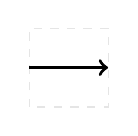
\begin{tikzpicture}
                \draw[white!90!black,dashed] (0,0) rectangle (1,1);
                \draw[very thick,->] (0,0.5) -- (1,0.5);
            \end{tikzpicture}
        }
        \correctchoice{
            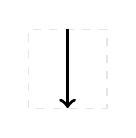
\begin{tikzpicture}
                \draw[white!90!black,dashed] (0,0) rectangle (1,1);
                \draw[very thick,->] (0.5,1) -- (0.5,0);
            \end{tikzpicture}
        }
        \wrongchoice{
            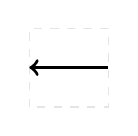
\begin{tikzpicture}
                \draw[white!90!black,dashed] (0,0) rectangle (1,1);
                \draw[very thick,->] (1,0.5) -- (0,0.5);
            \end{tikzpicture}
        }
        \wrongchoice{
            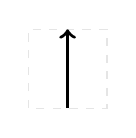
\begin{tikzpicture}
                \draw[white!90!black,dashed] (0,0) rectangle (1,1);
                \draw[very thick,->] (0.5,0) -- (0.5,1);
            \end{tikzpicture}
        }
        \wrongchoice{
            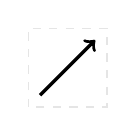
\begin{tikzpicture}
                \draw[white!90!black,dashed] (0,0) rectangle (1,1);
                \draw[very thick,->] (0.15,0.15) -- (0.85,0.85);
            \end{tikzpicture}
        }
    \end{choices}
    \end{multicols}
\end{question}
}

\element{njctl}{
\begin{question}{momentum-Q16}
    %% Questions 15-16
    A stationary cannon ball explodes in three pieces of masses $m$, $m$, and $2m$.
    The two momenta of the equal masses is presented by the diagram below.
    \begin{center}
        \PSIapcMomentumQFifteen
    \end{center}
    What is the magnitude of the velocity of the $2m$ cannon ball piece?
    \begin{multicols}{3}
    \begin{choices}
      \correctchoice{$\dfrac{\sqrt{2}}{2} v$}
        \wrongchoice{$\dfrac{\sqrt{3}}{2} v$}
        \wrongchoice{$\dfrac{\sqrt{5}}{2} v$}
        \wrongchoice{$\dfrac{1}{2} v$}
        \wrongchoice{$\dfrac{3}{2} v$}
    \end{choices}
    \end{multicols}
\end{question}
}

%\element{njctl}{
%\begin{question}{momentum-Q17}
%    An object with an initial momentum, shown in the diagram below,
%        collides with another object at rest.
%    \begin{center}
%    \begin{tikzpicture}
%        \draw[very thick,->] (0,0) -- (3,0);
%    \end{tikzpicture}
%    \end{center}
%    Which of the following combinations of two vectors may represent the momenta of the two objects after the collision?
%    \begin{multicols}{3}
%    \begin{choices}
%        %% NOTE: ANS is E
%        %% TODO: tikz options
%        \AMCboxDimensions{down=-1cm}
%        \wrongchoice{
%            \begin{tikzpicture}
%                \draw[fill] (0,0) circle (1.5pt);
%                \draw[thick,->] (0,0) -- (0,1);
%                \draw[thick,->] (0,0) -- (0,-0.5);
%            \end{tikzpicture}
%        }
%    \end{choices}
%    \end{multicols}
%\end{question}
%}

\newcommand{\PSIapcMomentumQEighteen}{
\begin{tikzpicture}
    %% Ground
    \node[anchor=north,fill,pattern=north east lines,minimum width=7cm, minimum height=0.05cm] at (0.5,0) {};
    \draw (-3,0) -- (4,0);
    %% Mass
    \node[draw,fill=white!90!black,minimum size=1cm,anchor=south] (A) at (-2,0) {\SI{6}{\kilo\gram}};
    \node[draw,fill=white!90!black,minimum size=1cm,anchor=south] (B) at (+1.75,0) {\SI{6}{\kilo\gram}};
    \node[draw,fill=white!90!black,minimum size=1cm,anchor=south] (C) at (+3.25,0) {\SI{6}{\kilo\gram}};
    %% Vectors
    \draw[thick,->] (A.east) -- ++(0:1cm) node[anchor=south,pos=0.5] {\SI{5}{\meter\per\second}};
\end{tikzpicture}
}

\element{njctl}{
\begin{question}{momentum-Q18}
    %% Questions 18-19 tikz
    A \SI{6}{\kilo\gram} block moves with a constant speed of \SI{5}{\meter\per\second} on a horizontal frictionless surface and collides elastically with an identical block initially at rest.
    The second block then collides and sticks to the last \SI{6}{\kilo\gram} block initially at rest.
    \begin{center}
        \PSIapcMomentumQEighteen
    \end{center}
    What is the speed of the second \SI{6}{\kilo\gram} block after the first collision?
    \begin{multicols}{3}
    \begin{choices}
        \wrongchoice{zero}
        \wrongchoice{\SI{2}{\meter\per\second}}
        \wrongchoice{\SI{2.5}{\meter\per\second}}
        \wrongchoice{\SI{3}{\meter\per\second}}
      \correctchoice{\SI{5}{\meter\per\second}}
    \end{choices}
    \end{multicols}
\end{question}
}

\element{njctl}{
\begin{question}{momentum-Q19}
    %% Questions 18-19 tikz
    A \SI{6}{\kilo\gram} block moves with a constant speed of \SI{5}{\meter\per\second} on a horizontal frictionless surface and collides elastically with an identical block initially at rest.
    The second block then collides and sticks to the last \SI{6}{\kilo\gram} block initially at rest.
    \begin{center}
        \PSIapcMomentumQEighteen
    \end{center}
    What is the speed of the third \SI{6}{\kilo\gram} block after the second collision?
    \begin{multicols}{3}
    \begin{choices}
        \wrongchoice{zero}
        \wrongchoice{\SI{2}{\meter\per\second}}
      \correctchoice{\SI{2.5}{\meter\per\second}}
        \wrongchoice{\SI{3}{\meter\per\second}}
        \wrongchoice{\SI{5}{\meter\per\second}}
    \end{choices}
    \end{multicols}
\end{question}
}

\newcommand{\PSIcalculusMomentumQTwenty}{
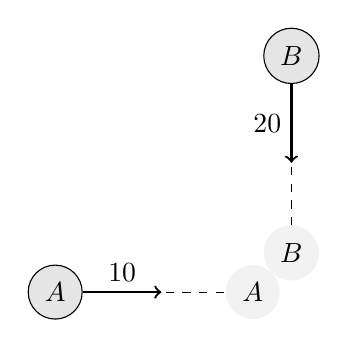
\begin{tikzpicture}
    %% Mass, Start
    \node[draw,circle,fill=white!90!black,minimum size=1em,anchor=center] (A) at (-3,0) {$A$};
    \node[draw,circle,fill=white!90!black,minimum size=1em,anchor=center] (B) at (0,+3) {$B$};
    %% Paths
    \draw[dashed] (A.east) -- (-1em,0);
    \draw[dashed] (B.south) -- (0,1em);
    %% Vectors
    \draw[thick,->] (A.east) -- ++(0:1cm) node[pos=0.5,anchor=south] {\SI{10}{\meter\per\second}};
    \draw[thick,->] (B.south) -- ++(270:1cm) node[pos=0.5,anchor=east] {\SI{20}{\meter\per\second}};
    %% Mass, Stop
    \node[dashed,circle,fill=white!95!black,minimum size=1em,anchor=east] (AF) at (-0.4em,0) {$A$};
    \node[dashed,circle,fill=white!95!black,minimum size=1em,anchor=south] (BF) at (0,0.4em) {$B$};
\end{tikzpicture}
}

\element{njctl}{
\begin{question}{momentum-Q20}
    %% Questions 20-21 tikz
    Object $A$ with mass \SI{8}{\kilo\gram} travels to the east at \SI{10}{\meter\per\second} and object $B$ with mass \SI{3}{\kilo\gram} travels south at \SI{20}{\meter\per\second}.
    The two objects collide and stick together.
    \begin{center}
        \PSIcalculusMomentumQTwenty
    \end{center}
    What is the magnitude of the velocity they have after the collision?
    \begin{multicols}{3}
    \begin{choices}
        \wrongchoice{\SI{1.8}{\meter\per\second}}
        \wrongchoice{\SI{9.1}{\meter\per\second}}
      \correctchoice{\SI{12.7}{\meter\per\second}}
        \wrongchoice{\SI{20}{\meter\per\second}}
        \wrongchoice{\SI{25.5}{\meter\per\second}}
    \end{choices}
    \end{multicols}
\end{question}
}

\element{njctl}{
\begin{question}{momentum-Q21}
    %% Questions 20-21 tikz
    Object $A$ with mass \SI{8}{\kilo\gram} travels to the east at \SI{10}{\meter\per\second} and object $B$ with mass \SI{3}{\kilo\gram} travels south at \SI{20}{\meter\per\second}.
    The two objects collide and stick together.
    \begin{center}
        \PSIcalculusMomentumQTwenty
    \end{center}
    What is the direction of the velocity they have after the collision?
    \begin{multicols}{2}
    \begin{choices}
        \wrongchoice{\ang{30} south of east}
      \correctchoice{\ang{37} south of east}
        \wrongchoice{\ang{45} south of east}
        \wrongchoice{\ang{53} south of east}
        \wrongchoice{\ang{60} south of east}
    \end{choices}
    \end{multicols}
\end{question}
}

\element{njctl}{
\begin{question}{momentum-Q22}
    Two balls of equal mass $m$ move with equal speeds $v$ along paths inclined at \ang{30} from the horizontal as shown.
    \begin{center}
    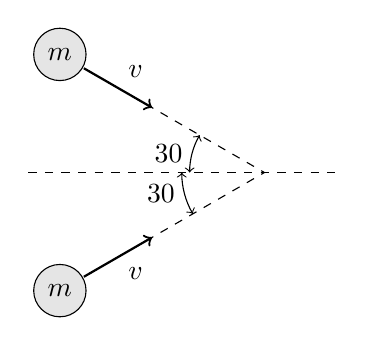
\begin{tikzpicture}
        %% Paths
        \draw[dashed] (-3,0) -- (1,0);
        \draw[dashed] (210:3) -- (0,0);
        \draw[dashed] (150:3) -- (0,0);
        %% Mass, Start
        \node[draw,circle,fill=white!90!black,minimum size=1em,anchor=center] (A) at (210:3) {$m$};
        \node[draw,circle,fill=white!90!black,minimum size=1em,anchor=center] (B) at (150:3) {$m$};
        %% Angles
        \draw[<->] (-0.95,0) arc (180:150:0.95) node[pos=0.5,anchor=east] {\ang{30}};
        \draw[<->] (-1.05,0) arc (180:210:1.05) node[pos=0.5,anchor=east] {\ang{30}};
        %% Vectors
        \draw[thick,->] (A.center) ++(30:1em) -- ++(30:1cm) node[pos=0.5,anchor=north west] {$v$};
        \draw[thick,->] (B.center) ++(330:1em) -- ++(330:1cm) node[pos=0.5,anchor=south west] {$v$};
    \end{tikzpicture}
    \end{center}
    After the collision they stick together.
    What is the magnitude of their velocity after the collision?
    \begin{multicols}{3}
    \begin{choices}
        \wrongchoice{$\sqrt{2} v$}
        \wrongchoice{$\dfrac{v}{2}$}
        \wrongchoice{$\dfrac{\sqrt{2}v}{2}$}
      \correctchoice{$\dfrac{\sqrt{3}v}{2}$}
        \wrongchoice{$v$}
    \end{choices}
    \end{multicols}
\end{question}
}

\element{njctl}{
\begin{question}{momentum-Q23}
    Block $m_1$ is moving with speed $v_0$ towards a stationary block $m_2$,
        then collides and sticks to it.
    After the collision, the speed of the center of mass of the system is:
    \begin{multicols}{2}
    \begin{choices}
        \wrongchoice{$\dfrac{m_1}{m_2} v_0$}
        \wrongchoice{$\dfrac{m_2+m_1}{m_2} v_0$}
        \wrongchoice{$\dfrac{m_2+m_1}{m_1} v_0$}
        \wrongchoice{$\left(1+m_2\right) v_0$}
      \correctchoice{$\dfrac{m_1}{m_1+m_2} v_0$}
    \end{choices}
    \end{multicols}
\end{question}
}

\element{njctl}{
\begin{question}{momentum-Q24}
    A cannonball of mass $2m$ is moving towards the right with initial velocity $v_0$,
        and explodes into two equal pieces each with mass $m$.
    What is the speed of the center of mass after the explosion?
    \begin{multicols}{3}
    \begin{choices}
      \correctchoice{$v_0$}
        \wrongchoice{$\dfrac{1}{2} v_0$}
        \wrongchoice{$2 v_0$}
        \wrongchoice{$4 v_0$}
        \wrongchoice{zero}
    \end{choices}
    \end{multicols}
\end{question}
}

\element{njctl}{
\begin{question}{momentum-Q25}
    A bullet of mass $M_1$ is fired from a gun that is initially at rest.
    The combined mass of the gun and bullet is $M_2$.
    If after the bullet is fired its kinetic energy is $KE$,
        what is the kinetic energy of the gun when it recoils?
    \begin{multicols}{2}
    \begin{choices}
        \wrongchoice{$KE$}
        \wrongchoice{$\dfrac{M_2}{M_1} KE$}
        \wrongchoice{$\dfrac{M_2^2}{M_1^2} KE$}
      \correctchoice{$\dfrac{M_1}{M_2-M_1} KE$}
        \wrongchoice{$\sqrt{\dfrac{M_1}{M_2-M_1}} KE$}
    \end{choices}
    \end{multicols}
\end{question}
}

\element{njctl}{
\begin{question}{momentum-Q26}
    A ball of mass $m$ is moving to the right with speed $3v$ on a frictionless tabletop when it collides with a second ball of mass $3m$ that is moving to the right with speed $v$.
    \begin{center}
    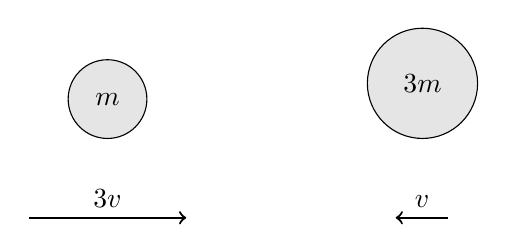
\begin{tikzpicture}
        %% Mass
        \node[draw,circle,fill=white!90!black,minimum size=1.0cm,anchor=south] (A) at (-2,0) {$m$};
        \node[draw,circle,fill=white!90!black,minimum size=1.4cm,anchor=south] (B) at (+2,0) {$3m$};
        %% Vectors
        \draw[thick,->] (-3,-1) -- (-1,-1) node[pos=0.5,anchor=south] {$3v$};
        \draw[thick,->] (+2.33,-1) -- (+1.66,-1) node[pos=0.5,anchor=south] {$v$};
    \end{tikzpicture}
    \end{center}
    If the two balls stick together upon impact the speed of the balls immediately after the collision is:
    \begin{multicols}{3}
    \begin{choices}
        \wrongchoice{$\dfrac{v}{3}$}
        \wrongchoice{$\dfrac{v}{2}$}
        \wrongchoice{$\dfrac{2v}{3}$}
      \correctchoice{$\dfrac{3v}{2}$}
        \wrongchoice{$2v$}
    \end{choices}
    \end{multicols}
\end{question}
}

\element{njctl}{
\begin{question}{momentum-Q27}
    Person $A$ and Person $B$ are standing on a sheet of frictionless ice.
    Person $A$ pushes Person $B$ so that Person $B$ who is \SI{60}{\kilo\gram},
        moves to the right at \SI{3}{\meter\per\second},
        while Person $A$, who is \SI{90}{\kilo\gram},
        moves to the left at \SI{2}{\meter\per\second}.
    What is the velocity of their center of mass?
    \begin{multicols}{2}
    \begin{choices}
      \correctchoice{zero}
        \wrongchoice{\SI{0.5}{\meter\per\second} to the left}
        \wrongchoice{\SI{2.4}{\meter\per\second} to the left}
        \wrongchoice{\SI{1}{\meter\per\second} to the right}
        \wrongchoice{\SI{2.5}{\meter\per\second} to the right}
    \end{choices}
    \end{multicols}
\end{question}
}

\element{njctl}{
\begin{question}{momentum-Q28}
    What is the rebound speed of a \SI{4}{\kilo\gram} ball falling straight down that hits a platform at \SI{4}{\meter\per\second},
        if the average normal force exerted by the platform on the ball is \SI{40}{\newton} for \SI{0.5}{\second}?
    \begin{multicols}{3}
    \begin{choices}
        \wrongchoice{\SI{2}{\meter\per\second}}
        \wrongchoice{\SI{7}{\meter\per\second}}
        \wrongchoice{\SI{6}{\meter\per\second}}
        \wrongchoice{\SI{9}{\meter\per\second}}
      \correctchoice{\SI{1}{\meter\per\second}}
    \end{choices}
    \end{multicols}
\end{question}
}

\element{njctl}{
\begin{question}{momentum-Q29}
    A \SI{2}{\kilo\gram} mass moving at \SI{12}{\meter\per\second} collides with an identical mass moving at \SI{-8}{\meter\per\second} and the masses stick together.
    What is the final velocity of the two masses?
    \begin{multicols}{3}
    \begin{choices}
        \wrongchoice{\SI{4/3}{\meter\per\second}}
      \correctchoice{\SI{2}{\meter\per\second}}
        \wrongchoice{\SI{6}{\meter\per\second}}
        \wrongchoice{\SI{10}{\meter\per\second}}
        \wrongchoice{\SI{12}{\meter\per\second}}
    \end{choices}
    \end{multicols}
\end{question}
}

\element{njctl}{
\begin{question}{momentum-Q30}
    A compressed spring is placed between two masses $M$ and $m$ resting on a smooth horizontal surface.
    When the spring is released,
        the two fly apart with $M$ moving at velocity $v$.
    The velocity of $m$ is:
    \begin{multicols}{3}
    \begin{choices}
        \wrongchoice{$\dfrac{M}{m} v$}
      \correctchoice{$-\dfrac{M}{m} v$}
        \wrongchoice{$\dfrac{m}{M} v$}
        \wrongchoice{$-\dfrac{m}{M} v$}
        \wrongchoice{$\dfrac{m}{m+M} v$}
    \end{choices}
    \end{multicols}
\end{question}
}

\element{njctl}{
\begin{question}{momentum-Q31}
    Consider these two cases:
    \emph{First}, a car moving at \SI{40}{\mile\per\hour} hits another car of equal mass moving at \SI{40}{\mile\per\hour} in the opposite direction.
    \emph{Second}, a car moving at \SI{40}{\mile\per\hour} hits a stationary steel wall.
    The collision time is the same for the two cases and the collisions are both inelastic.
    In which of these cases would result in the greatest impact force?
    \begin{choices}
        \wrongchoice{Hitting the wall}
        \wrongchoice{Hitting the other car}
        %% MISTAKE: the force would be equal, F = \Delta p / \Delta t
      \correctchoice{The force would be the same in both cases}
        \wrongchoice{More information is needed}
        \wrongchoice{None of the provided are true}
    \end{choices}
\end{question}
}

\element{njctl}{
\begin{question}{momentum-Q32}
    %% Questions 32-33
    A mass $M$ moving with speed $v$ collides with an uncompressed stationary spring of mass $M$ with a spring constant $K$.
    The surface is frictionless.
    %% Begin question
    What will be the maximum compression of the spring?
    \begin{multicols}{3}
    \begin{choices}
        \wrongchoice{$v\sqrt{\dfrac{M}{K}}$}
        \wrongchoice{$v\sqrt{\dfrac{M}{4K}}$}
        %% NOTE: dup of B??
        \wrongchoice{$\dfrac{v}{2}\sqrt{\dfrac{M}{K}}$}
        \wrongchoice{$v \sqrt{\dfrac{2M}{K}}$}
      \correctchoice{$v \sqrt{\dfrac{M}{2K}}$}
    \end{choices}
    \end{multicols}
\end{question}
}

\element{njctl}{
\begin{question}{momentum-Q33}
    %% Questions 32-33
    A mass $M$ moving with speed $v$ collides with an uncompressed stationary spring of mass $M$ with a spring constant $K$.
    The surface is frictionless.
    %% Begin question
    What is the speed of the spring after the collision?
    \begin{multicols}{3}
    \begin{choices}
        \wrongchoice{$v$}
      \correctchoice{$\dfrac{v}{2}$}
        \wrongchoice{$\dfrac{v}{4}$}
        \wrongchoice{$2v$}
        \wrongchoice{$\dfrac{v}{3}$}
    \end{choices}
    \end{multicols}
\end{question}
}

\newcommand{\PSIcalculusMomentumQThirtyFour}{
\begin{tikzpicture}
    \begin{axis}[
        axis y line=left,
        axis x line=bottom,
        axis line style={->},
        xlabel={time},
        x unit=\si{\second},
        xtick={0,2,4,6,8},
        minor x tick num=1,
        ylabel={force},
        y unit=\si{\newton},
        ytick={0,2,4,6},
        minor y tick num=1,
        xmin=0,xmax=8.25,
        ymin=0,ymax=6.25,
        width=0.8\columnwidth,
        height=0.5\columnwidth,
        grid=both,
        very thin,
    ]
    \addplot[line width=1pt,mark=\empty] plot coordinates {(0,0) (2,6) (6,6) (8,0)};
    \end{axis}
\end{tikzpicture}
}

\element{njctl}{
\begin{question}{momentum-Q34}
    %% Questions 34-35 pgfplots
    A \SI{6}{\kilo\gram} mass moving at \SI{12}{\meter\per\second} in the $+x$ direction is acted upon by a force with magnitude given as a function of time by the below graph.
    \begin{center}
        \PSIcalculusMomentumQThirtyFour
    \end{center}
    %% Start question
    Find the magnitude of the change in momentum from time $t=0$ to time $t=\SI{8}{\second}$.
    \begin{multicols}{2}
    \begin{choices}
        \wrongchoice{\SI{12}{\kilo\gram\meter\per\second}}
        \wrongchoice{\SI{24}{\kilo\gram\meter\per\second}}
      \correctchoice{\SI{36}{\kilo\gram\meter\per\second}}
        \wrongchoice{\SI{40}{\kilo\gram\meter\per\second}}
        \wrongchoice{\SI{52}{\kilo\gram\meter\per\second}}
    \end{choices}
    \end{multicols}
\end{question}
}

\element{njctl}{
\begin{question}{momentum-Q35}
    %% Questions 34-35 pgfplots
    A \SI{6}{\kilo\gram} mass moving at \SI{12}{\meter\per\second} in the $+x$ direction is acted upon by a force with magnitude given as a function of time by the below graph.
    \begin{center}
        \PSIcalculusMomentumQThirtyFour
    \end{center}
    %% Start question
    What is the velocity of the mass after the force has stopped acting?
    \begin{multicols}{3}
    \begin{choices}
        \wrongchoice{\SI{6}{\meter\per\second}}
        \wrongchoice{\SI{10}{\meter\per\second}}
      \correctchoice{\SI{18}{\meter\per\second}}
        \wrongchoice{\SI{24}{\meter\per\second}}
        \wrongchoice{\SI{40}{\meter\per\second}}
    \end{choices}
    \end{multicols}
\end{question}
}

\element{njctl}{
\begin{question}{momentum-Q36}
    A wire is bent into the shape as shown below.
    \begin{center}
    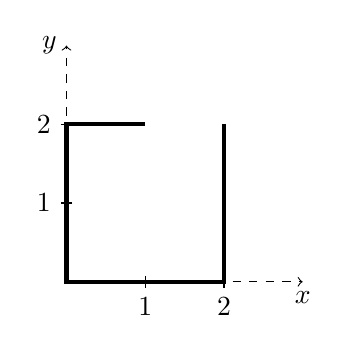
\begin{tikzpicture}
        %% Axis
        \draw[dashed,->] (0,0) -- (0,3) node[anchor=east] {$y$};
        \draw[dashed,->] (0,0) -- (3,0) node[anchor=north] {$x$};
        %% Labels
        \foreach \i in {1,2} {
            \draw (\i,0.5ex) -- (\i,-0.5ex) node[anchor=north] {\i};
            \draw (0.5ex,\i) -- (-0.5ex,\i) node[anchor=east] {\i};
        }
        %% Wire
        \draw[ultra thick] (1,2) --  (0,2) -- (0,0) -- (2,0) -- (2,2);
    \end{tikzpicture}
    \end{center}
    Which of the following best represents the coordinates of the center of mass?
    \begin{multicols}{3}
    \begin{choices}
      \correctchoice{$\left(\dfrac{13}{14}, \dfrac{6}{7}\right)$}
        \wrongchoice{$\left(\dfrac{8}{7},   \dfrac{6}{7}\right)$}
        \wrongchoice{$\left(\dfrac{13}{14}, \dfrac{8}{7}\right)$}
        \wrongchoice{$\left(1,1\right)$}
        \wrongchoice{$\left(1,\dfrac{6}{7}\right)$}
    \end{choices}
    \end{multicols}
\end{question}
}

\element{njctl}{
\begin{question}{momentum-Q37}
    A block of mass $m$ is moving with speed $v_0$ to the right on a frictionless surface when it explodes into two pieces of unequal mass.
    \begin{center}
    \begin{tikzpicture}
        %% Ground
        \node[anchor=north,fill,pattern=north east lines,minimum width=6cm, minimum height=0.05cm] at (0,0) {};
        \draw (-3,0) -- (3,0);
        %% Mass
        \node[draw,fill=white!90!black,minimum size=1cm,anchor=south] (A) at (-1,0) {$m$};
        %% Velocity
        \draw[very thick,->] (A.east) -- ++(0:1.5cm) node[pos=0.5,anchor=south] {$v_0$};
    \end{tikzpicture}
    \end{center}
    One piece of the mass,
        $\dfrac{3m}{4}$ moves with a speed $\dfrac{v_0}{2}$ to the left while the other piece of the object moves with velocity:
    \begin{multicols}{3}
    \begin{choices}
        \wrongchoice{$\dfrac{v_0}{2}$}
        \wrongchoice{$\dfrac{2v_0}{3}$}
      \correctchoice{$\dfrac{11v_0}{2}$}
        \wrongchoice{$\dfrac{7v_0}{5}$}
        \wrongchoice{$2v_0$}
    \end{choices}
    \end{multicols}
\end{question}
}

\element{njctl}{
\begin{question}{momentum-Q38}
    Two blocks with masses $m$ and $2m$ are placed on a horizontal frictionless surface.
    There is a compressed spring between the block and after the spring is released,
        the $2m$ block moves to the right with a speed of $v$.
    \begin{center}
    \begin{tikzpicture}
        %% Ground
        \node[anchor=north,fill,pattern=north east lines,minimum width=6cm, minimum height=0.05cm] at (0,0) {};
        \draw (-3,0) -- (3,0);
        %% Two Mass
        \node[draw,fill=white!90!black,minimum size=1cm,anchor=south] (A) at (-1.5,0) {$m$};
        \node[draw,fill=white!90!black,minimum height=1cm,minimum width=1.5cm,anchor=south] (B) at (+1.5,0) {$2m$};
        %% Vector
        \draw[thick,->] (B.east) -- ++(0:1.5cm) node[anchor=south,pos=0.5] {$v$};
        %% Spring
        \draw[thick,decoration={aspect=0.2,segment length=2.0mm,amplitude=3mm,coil},decorate] (A.east) -- (B.west);
    \end{tikzpicture}
    \end{center}
    What is the total work done by the spring on the system of two blocks?
    \begin{multicols}{3}
    \begin{choices}
        \wrongchoice{zero}
        \wrongchoice{$mv^2$}
        \wrongchoice{$2mv^2$}
      \correctchoice{$3mv^2$}
        \wrongchoice{$mv$}
    \end{choices}
    \end{multicols}
\end{question}
}

\element{njctl}{
\begin{question}{momentum-Q39}
    A railway artillery gun of mass \SI{1400}{\mega\gram} is initially at rest on a horizontal surface.
    It fires a \SI{7}{\mega\gram} shell with a velocity of \SI{800}{\meter\per\second} at an angle of \ang{60}.
        What is the speed of the gun immediately after the shell is fired?
    \begin{multicols}{3}
    \begin{choices}
        \wrongchoice{Zero}
      \correctchoice{\SI{2}{\meter\per\second}}
        \wrongchoice{\SI{4}{\meter\per\second}}
        \wrongchoice{\SI{5}{\meter\per\second}}
        \wrongchoice{\SI{7}{\meter\per\second}}
    \end{choices}
    \end{multicols}
\end{question}
}

\element{njctl}{
\begin{question}{momentum-Q40}
    Two equal forces are exerted for the same length of time on two blocks with different masses $m_1$ and $m_2$ ($m_2>m_1$).
    Which of the following will describe the change is kinetic energy of the blocks?
    \begin{choices}
        \wrongchoice{The blocks have the same change in kinetic energy.}
        \wrongchoice{The change in kinetic energy of each block is zero.}
        \wrongchoice{Block $m_2$ has a greater change in kinetic energy.}
      \correctchoice{Block $m_1$ has a greater change in kinetic energy.}
        \wrongchoice{None of the provided are correct.}
    \end{choices}
\end{question}
}

\element{njctl}{
\begin{question}{momentum-Q41}
    A boy launches a \SI{20}{\gram} dart horizontally by a spring gun from a balcony \SI{45}{\meter} above the ground.
    The dart lands \SI{15}{\meter} away from the balcony.
    If the length of the gun's barrel is \SI{10}{\centi\meter},
        what is the average horizontal force applied by the spring?
    \begin{multicols}{3}
    \begin{choices}
        \wrongchoice{\SI{1.0}{\newton}}
        \wrongchoice{\SI{2.0}{\newton}}
      \correctchoice{\SI{2.5}{\newton}}
        \wrongchoice{\SI{5.0}{\newton}}
        \wrongchoice{\SI{7.5}{\newton}}
    \end{choices}
    \end{multicols}
\end{question}
}

\element{njctl}{
\begin{question}{momentum-Q42}
    A ball of mass $m$ is dropped from a height of $h_0$.
    The ball hits the floor and bounces to a height of $h$.
    What is the magnitude of impulse exerted on the ball by the floor?
    %\begin{multicols}{2}
    \begin{choices}
        \wrongchoice{$mgh$}
        \wrongchoice{$2mgh$}
        \wrongchoice{$\sqrt{2mgh}$}
      \correctchoice{$m\left(\sqrt{2gh} + \sqrt{2gh_0}\right)$}
        \wrongchoice{$m\left(\sqrt{2gh} - \sqrt{2gh_0}\right)$}
    \end{choices}
    %\end{multicols}
\end{question}
}

\element{njctl}{
\begin{question}{momentum-Q43}
    A \SI{5}{\kilo\gram} object starts from rest on a flat horizontal surface and moves in a straight line.
    The velocity as a function of time is given by $v=3t+2t^2$.
    What is the magnitude of the instantaneous force that acts on the object at \SI{2}{\second}?
    \begin{multicols}{3}
    \begin{choices}
        \wrongchoice{\SI{105}{\newton}}
        \wrongchoice{\SI{75}{\newton}}
      \correctchoice{\SI{55}{\newton}}
        \wrongchoice{\SI{45}{\newton}}
        \wrongchoice{\SI{35}{\newton}}
    \end{choices}
    \end{multicols}
\end{question}
}

\element{njctl}{
\begin{question}{momentum-Q44}
    A net force $F=10+6t^2$ is applied to a \SI{30}{\kilo\gram} cart that can move on a flat horizontal surface.
    If the cart starts from rest,
        what is its speed at \SI{5}{\second}?
    \begin{multicols}{3}
    \begin{choices}
      \correctchoice{\SI{10}{\meter\per\second}}
        \wrongchoice{\SI{8}{\meter\per\second}}
        \wrongchoice{\SI{5}{\meter\per\second}}
        \wrongchoice{\SI{3}{\meter\per\second}}
        \wrongchoice{\SI{1}{\meter\per\second}}
    \end{choices}
    \end{multicols}
\end{question}
}

\element{njctl}{
\begin{question}{momentum-Q45}
    A block of mass $m$ moves to the right at a constant velocity $v$ and collides elastically with another block of mass $3m$,
        which is initially at rest.
    \begin{center}
    \begin{tikzpicture}
        %% Ground
        \node[anchor=north,fill,pattern=north east lines,minimum width=6cm, minimum height=0.05cm] at (0,0) {};
        \draw (-3,0) -- (3,0);
        %% Mass
        \node[draw,fill=white!90!black,minimum size=1cm,anchor=south] (A) at (-2,0) {$m$};
        \node[draw,fill=white!90!black,minimum size=1.4cm,anchor=south] (B) at (+2,0) {$3m$};
        %% Vectors
        \draw[thick,->] (A.east) -- ++(0:1cm) node[anchor=south,pos=0.5] {$v$};
    \end{tikzpicture}
    \end{center}
    Which of the following is the velocity of each block after the collision?
    \begin{multicols}{2}
    \begin{choices}
        \wrongchoice{$v_m=\text{zero}$, $v_{3m}=v$}
        \wrongchoice{$v_m=\dfrac{v}{2}$, $v_{3m}=\dfrac{v}{2}$}
      \correctchoice{$v_m=-\dfrac{v}{2}$, $v_{3m}=\dfrac{v}{2}$}
        \wrongchoice{$v_m=\dfrac{3v}{2}$, $v_{3m}=\dfrac{v}{2}$}
        \wrongchoice{$v_m=-\dfrac{v}{2}$, $v_{3m}=\dfrac{3v}{2}$}
    \end{choices}
    \end{multicols}
\end{question}
}

\element{njctl}{
\begin{question}{momentum-Q46}
    A \SI{40}{\kilo\gram} skateboarder runs at a constant velocity of \SI{12}{\meter\per\second} and jumps on a stationary skateboard with a mass of \SI{8}{\kilo\gram}.
    %% NOTE: diagram not needed
    What is the velocity of the skateboarder--skateboard system after the jump?
    \begin{multicols}{3}
    \begin{choices}
        \wrongchoice{\SI{12}{\meter\per\second}}
        \wrongchoice{\SI{90}{\meter\per\second}}
        \wrongchoice{\SI{60}{\meter\per\second}}
        \wrongchoice{\SI{20}{\meter\per\second}}
      \correctchoice{\SI{10}{\meter\per\second}}
    \end{choices}
    \end{multicols}
\end{question}
}

\element{njctl}{
\begin{question}{momentum-Q47}
    An \SI{80}{\kilo\gram} diver jumps off a moving boat.
    The boat has a mass of \SI{400}{\kilogram} and moves at a constant velocity of \SI{2}{\meter\per\second}.
    %% NOTE: diagram not needed
    What is the velocity of the boat after the jump if the diver jumps with a velocity of \SI{3}{\meter\per\second} in opposite direction to the initial velocity of the boat?
    \begin{multicols}{3}
    \begin{choices}
        \wrongchoice{\SI{2}{\meter\per\second}}
      \correctchoice{\SI{3}{\meter\per\second}}
        \wrongchoice{\SI{4}{\meter\per\second}}
        \wrongchoice{\SI{5}{\meter\per\second}}
        \wrongchoice{\SI{6}{\meter\per\second}}
    \end{choices}
    \end{multicols}
\end{question}
}

\element{njctl}{
\begin{question}{momentum-Q48}
    A tennis ball approaches a racket with a momentum of \SI{5}{\kilo\gram\meter\per\second} and bounces back with a momentum of \SI{6}{\kilo\gram\meter\per\second} after the collision with the racket.
    \begin{center}
    \begin{tikzpicture}
        %% Before
        \node[draw,circle,fill=white!90!black,minimum size=1em,anchor=south] (A) at (-1.5,0) {};
        \node[anchor=north] at (A.south) {Before};
        \draw[thick,->] (A.west) -- ++(180:1.5cm) node[pos=0.5,anchor=south] {\SI{5}{\kilo\gram\meter\per\second}};
        %% After
        \node[draw,circle,fill=white!90!black,minimum size=1em,anchor=south] (B) at (+1.5,0) {};
        \node[anchor=north] at (B.south) {After};
        \draw[thick,->] (B.east) -- ++(0:1.5cm) node[pos=0.5,anchor=south] {\SI{6}{\kilo\gram\meter\per\second}};
    \end{tikzpicture}
    \end{center}
    What is the change in momentum of the tennis ball?
    \begin{multicols}{3}
    \begin{choices}
        \wrongchoice{\SI{1}{\kilo\gram\meter\per\second}}
        \wrongchoice{\SI{5}{\kilo\gram\meter\per\second}}
        \wrongchoice{\SI{6}{\kilo\gram\meter\per\second}}
      \correctchoice{\SI{11}{\kilo\gram\meter\per\second}}
        \wrongchoice{\SI{0}{\kilo\gram\meter\per\second}}
    \end{choices}
    \end{multicols}
\end{question}
}

\element{njctl}{
\begin{question}{momentum-Q49}
    A light beach ball moving with a velocity \SI{2}{\meter\per\second} to the right collides elastically with a stationary bowling ball.
    After the collision the bowling ball remains stationary.
    \begin{center}
    \begin{tikzpicture}
        %% Ground
        \node[anchor=north,fill,pattern=north east lines,minimum width=6cm, minimum height=0.05cm] at (0,0) {};
        \draw (-3,0) -- (3,0);
        %% Mass
        \node[draw,circle,fill=white!90!black,minimum size=1.4cm,anchor=south] (A) at (-2,0) {};
        \node[draw,circle,fill=white!90!black,minimum size=1cm,anchor=south] (B) at (+2,0) {};
        %% Vectors
        \draw[thick,->] (A.east) -- ++(0:1.5cm) node[anchor=south,pos=0.5] {\SI{2}{\meter\per\second}};
    \end{tikzpicture}
    \end{center}
    What is the velocity of the beach ball after the collision?
    \begin{multicols}{2}
    \begin{choices}
        \wrongchoice{zero}
      \correctchoice{\SI{2}{\meter\per\second} to the left}
        \wrongchoice{\SI{4}{\meter\per\second} to the left}
        \wrongchoice{\SI{3}{\meter\per\second} to the left}
        \wrongchoice{\SI{1}{\meter\per\second} to the left}
    \end{choices}
    \end{multicols}
\end{question}
}

\element{njctl}{
\begin{question}{momentum-Q50}
    A ball of mass $m$ moving at a constant speed $v$ to the right collides elastically with another ball of mass $3m$ moving to the left at a constant speed $v$.
    \begin{center}
    \begin{tikzpicture}
        %% Ground
        \node[anchor=north,fill,pattern=north east lines,minimum width=6cm, minimum height=0.05cm] at (0,0) {};
        \draw (-3,0) -- (3,0);
        %% Mass
        \node[draw,circle,fill=white!90!black,minimum size=1cm,anchor=south] (A) at (-2,0) {$m$};
        \node[draw,circle,fill=white!90!black,minimum size=1.4cm,anchor=south] (B) at (+2,0) {$3m$};
        %% Vectors
        \draw[thick,->] (A.east) -- ++(0:1cm) node[anchor=south,pos=0.5] {$v$};
        \draw[thick,->] (B.west) -- ++(180:1cm) node[anchor=south,pos=0.5] {$v$};
    \end{tikzpicture}
    \end{center}
    What is the velocity of ball $m$ after the collision?
    \begin{multicols}{3}
    \begin{choices}
        \wrongchoice{$v$}
        \wrongchoice{$-\dfrac{3v}{2}$}
        \wrongchoice{$-\dfrac{v}{3}$}
      \correctchoice{$-2v$}
        \wrongchoice{$3v$}
    \end{choices}
    \end{multicols}
\end{question}
}


\endinput



